\documentclass[a4paper]{scrreprt}

%% Language and font encodings
\usepackage[german]{babel}
\setcounter{secnumdepth}{3} 
\setcounter{tocdepth}{3} 
\usepackage[utf8x]{inputenc}
\usepackage[T1]{fontenc}
\usepackage{courier}
\usepackage{colortbl} 

%% Sets page size and margins
\usepackage[a4paper,top=3cm,bottom=2cm,left=3cm,right=3cm,marginparwidth=1.75cm]{geometry}

%% Useful packages
\usepackage{amsmath}
\usepackage{graphicx}
\usepackage[colorinlistoftodos]{todonotes}
\usepackage[colorlinks=true, allcolors=blue, breaklinks = true]{hyperref}
\usepackage{tocstyle}
\usetocstyle{standard}
\settocfeature{raggedhook}{\raggedright}
\usepackage{longtable}
\usepackage{scrhack}
\usepackage{graphicx}
\usepackage{float}
\graphicspath{ {images/} }

\begin{document}	
	\begin{flushright}
		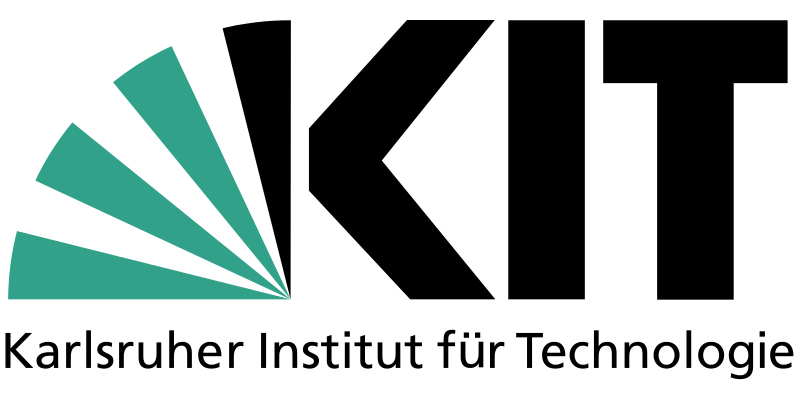
\includegraphics[scale = 0.2]{kit-logo.png}\\[0.5cm]
	\end{flushright}
	\vspace*{2cm}
	
	\begin{center}
		\large Praxis der Softwareentwicklung
		\vspace*{1.5cm}
		
		\textbf{\huge Fridget}
		\vspace*{1cm}
		
		\textbf{\Large Qualitätssicherung Testbericht}
		\vspace*{2cm}
		
		Yunjia Chen, Jasmin Jat, Min Hye Park, Alina Shah, Lisa Wang
		\vspace*{1cm}
		
		\today
		\vspace*{2.5cm}
		
		Betreuung: Erik Burger, Sandro Koch\\[0.5cm]
		IPD\\[0.5cm]
		
		Karlsruher Institut für Technologie
		
	\end{center}

	\thispagestyle{empty}
	
	\tableofcontents
	
	\chapter{Einleitung}
	Dies ist das Dokument für die Qualitätssicherung der Applikation Fridget – entstanden im Rahmen
	des Softwarepraktikums PSE im Sommersemester 2018.
	Zunächst verlieren wir in diesen Dokument Worte über die gefundenen Bugs in unserer App und wie wir diese beheben würden.
	In Abschnitt 2 beschreiben wir die Änderungen gegenüber des Feinentwurfs.
	Ebenso wichtig sind die Unit Tests der Applikation, welche im nachfolgenden Abschnitt 4 aufgelistet sind.
	
	\chapter{Gefundene Bugs und deren Behebung}
	Folgende Bugs wurden gefunden:
	\begin{flushleft}
		\begin{longtable}{|p{.32\textwidth}|p{.32\textwidth}|p{.32\textwidth}|}
		\hline
		\textbf{Fehlersymptom} & \textbf{Fehlergrund} & \textbf{Fehlerbehebung} \\
		\hline	
		\textbf{Editierung von Frozen Note wird überschrieben, wenn zwei Leute gleichzeitig editieren
		} & \textbf{EditFrozenNoteActivity wird nicht geblockt, wenn ein User drin ist} & \textbf{} \\
		\hline
		\end{longtable}
	\end{flushleft}	
	
	\chapter{Unit Tests}
	\section{Client}
	\subsection{Activity}
	\subsubsection{public class LoginActivityTest}
	\textbf{Beschreibung}\\
	\textit{Diese Klasse testet das erfolgreiche Builden der LoginActivity.}\\
	\\	
	\textbf{Methoden}
	\begin{itemize}
		
		\item\texttt{{public void setUp() throws Exception}}
		
		\textit{Diese Methode setzt die ActivityTestRule zur LoginActivity auf null.}
		
		\item\texttt{{public void TestLaunch()}}
		
		\textit{Diese Methode testet das Builden der View zur LoginActivity.}
		
		\item\texttt{{public void tearDown()}}
		
		\textit{Diese Methode setzt die ActivityTestRule zur LoginActivity wieder auf null.}
		
		
	\end{itemize}
	\subsubsection{public class StartActivityTest}
	\textbf{Beschreibung}\\
	\textit{Diese Klasse testet das erfolgreiche Builden der StartActivity.}\\
	\\	
	\textbf{Methoden}
	\begin{itemize}
		
		\item\texttt{{public void setUp() throws Exception}}
		
		\textit{Diese Methode setzt die ActivityTestRule zur StartActivity auf null.}
		
		\item\texttt{{public void TestLaunch()}}
		
		\textit{Diese Methode testet das Builden der View zur StartActivity.}
		
		\item\texttt{{public void tearDown()}}
		
		\textit{Diese Methode setzt die ActivityTestRule zur StartActivity wieder auf null.}
		
		
	\end{itemize}
	\subsubsection{public class HomeActivityTest}
	\textbf{Beschreibung}\\
	\textit{Diese Klasse testet das erfolgreiche Builden der HomeActivity.}\\
	\\	
	\textbf{Methoden}
	\begin{itemize}
		
		\item\texttt{{public void setUp() throws Exception}}
		
		\textit{Diese Methode setzt die ActivityTestRule zur HomeActivity auf null.}
		
		\item\texttt{{public void TestLaunch()}}
		
		\textit{Diese Methode testet das Builden der View zur HomeActivity.}
		
		\item\texttt{{public void tearDown()}}
		
		\textit{Diese Methode setzt die ActivityTestRule zur HomeActivity wieder auf null.}
		
		
	\end{itemize}
	\subsubsection{public class CreateFlatshareActivityTest}
	\textbf{Beschreibung}\\
	\textit{Diese Klasse testet das erfolgreiche Builden der CreateFlatshareActivity.}\\
	\\	
	\textbf{Methoden}
	\begin{itemize}
		
		\item\texttt{{public void setUp() throws Exception}}
		
		\textit{Diese Methode setzt die ActivityTestRule zur CreateFlatshareActivity auf null.}
		
		\item\texttt{{public void TestLaunch()}}
		
		\textit{Diese Methode testet das Builden der View zur CreateFlatshareActivity.}
		
		\item\texttt{{public void tearDown()}}
		
		\textit{Diese Methode setzt die ActivityTestRule zur CreateFlatshareActivity wieder auf null.}
		
		
	\end{itemize}
	\subsubsection{public class CreateTextCoolNoteActivityTest}
	\textbf{Beschreibung}\\
	\textit{Diese Klasse testet das erfolgreiche Builden der CreateTextCoolNoteActivity.}\\
	\\	
	\textbf{Methoden}
	\begin{itemize}
		
		\item\texttt{{public void setUp() throws Exception}}
		
		\textit{Diese Methode setzt die ActivityTestRule zur CreateTextCoolNoteActivity auf null.}
		
		\item\texttt{{public void TestLaunch()}}
		
		\textit{Diese Methode testet das Builden der View zur CreateTextCoolNoteActivity.}
		
		\item\texttt{{public void tearDown()}}
		
		\textit{Diese Methode setzt die ActivityTestRule zur CreateTextCoolNoteActivity wieder auf null.}
		
		
	\end{itemize}
	\subsubsection{public class EditTextFrozenNoteActivityTest}
	\textbf{Beschreibung}\\
	\textit{Diese Klasse testet das erfolgreiche Builden der EditTextFrozenNoteActivity.}\\
	\\	
	\textbf{Methoden}
	\begin{itemize}
		
		\item\texttt{{public void setUp() throws Exception}}
		
		\textit{Diese Methode setzt die ActivityTestRule zur EditTextFrozenNoteActivity auf null.}
		
		\item\texttt{{public void TestLaunch()}}
		
		\textit{Diese Methode testet das Builden der View zur EditTextFrozenNoteActivity.}
		
		\item\texttt{{public void tearDown()}}
		
		\textit{Diese Methode setzt die ActivityTestRule zur EditTextFrozenNoteActivity wieder auf null.}
		
		
	\end{itemize}
	\subsubsection{public class EnterAcccessCodeActivityTest}
	\textbf{Beschreibung}\\
	\textit{Diese Klasse testet das erfolgreiche Builden der EnterAccessCodeActivity.}\\
	\\	
	\textbf{Methoden}
	\begin{itemize}
		
		\item\texttt{{public void setUp() throws Exception}}
		
		\textit{Diese Methode setzt die ActivityTestRule zur EnterAccessCodeActivity auf null.}
		
		\item\texttt{{public void TestLaunch()}}
		
		\textit{Diese Methode testet das Builden der View zur EnterAccessCodeActivity.}
		
		\item\texttt{{public void tearDown()}}
		
		\textit{Diese Methode setzt die ActivityTestRule zur EnterAccessCodeActivity wieder auf null.}
		
		
	\end{itemize}
	\subsubsection{public class FullTextCoolNoteActivityTest}
	\textbf{Beschreibung}\\
	\textit{Diese Klasse testet das erfolgreiche Builden der FullTextCoolNoteActivity.}\\
	\\	
	\textbf{Methoden}
	\begin{itemize}
		
		\item\texttt{{public void setUp() throws Exception}}
		
		\textit{Diese Methode setzt die ActivityTestRule zur FullTextCoolNoteActivity auf null.}
		
		\item\texttt{{public void TestLaunch()}}
		
		\textit{Diese Methode testet das Builden der View zur FullTextCoolNoteActivity.}
		
		\item\texttt{{public void tearDown()}}
		
		\textit{Diese Methode setzt die ActivityTestRule zur FullTextCoolNoteActivity wieder auf null.}
		
		
	\end{itemize}
	\subsubsection{public class FullTextFrozenNoteActivityTest}
	\textbf{Beschreibung}\\
	\textit{Diese Klasse testet das erfolgreiche Builden der FullTextFrozenNoteActivity.}\\
	\\	
	\textbf{Methoden}
	\begin{itemize}
		
		\item\texttt{{public void setUp() throws Exception}}
		
		\textit{Diese Methode setzt die ActivityTestRule zur FullTextFrozenNoteActivity auf null.}
		
		\item\texttt{{public void TestLaunch()}}
		
		\textit{Diese Methode testet das Builden der View zur FullTextFrozenNoteActivity.}
		
		\item\texttt{{public void tearDown()}}
		
		\textit{Diese Methode setzt die ActivityTestRule zur FullTextFrozenNoteActivity wieder auf null.}
		
		
	\end{itemize}
	
	\subsection{Viewmodel}
	\subsubsection{public class StyledContentViewModelTest}
	\textbf{Beschreibung}\\
	\textit{Diese Klasse testet das Styling des Textes in der Content-Box.}\\
	\\	
	\textbf{Methoden}
	\begin{itemize}
		
		\item\texttt{{public void setUp() throws Exception}}
		
		\textit{Diese Methode erstellt ein neues StyledContentViewModel.}
		
		\item\texttt{{public void toggleBold\_ReturnsCorrectHtmlContent()}}
		
		\textit{Diese Methode testet den Bold-Button.}
		
		\item\texttt{{public void toggleItalic\_ReturnsCorrectHtmlContent()}}
		
		\textit{Diese Methode testet den Italic-Button.}
		
		\item\texttt{{public void toggleUnderline\_ReturnsCorrectHtmlContent()}}
		
		\textit{Diese Methode testet den Underline-Button.}
		
		\item\texttt{{public void toggleCombinedStyles\_ReturnsCorrectHtmlContent()}}
		
		\textit{Diese Methode testet die Kombination aus alles Styling-Button.}
		
		\item\texttt{{public void parseFromHtmlContent\_ReturnsTheSameHtmlContent()}}
		
		\textit{Diese Methode testet das Parsen des Textes.}
		
	\end{itemize}
	\subsection{Services}
	\subsubsection{\texttt{public class AccessCodeServiceTest}}
	\textbf{Beschreibung}\\
	\textit{Diese Klasse testet die Requests des Access-Code-Services.}\\
	\\	
	\textbf{Methoden}
	\begin{itemize}

		\item\texttt{{public void setUp() throws Exception}}
		
		\textit{Diese Methode baut die MockRetrofit-Instanz.}
		
		\item\texttt{{public void testGenerateAccesscode() throws Exception}}
		
		\textit{Diese Methode testet das Request zum Generieren eines Zugangscodes.}
		
		
	\end{itemize}
	\subsubsection{\texttt{public class CoolNoteServiceTest}}
	\textbf{Beschreibung}\\
	\textit{Diese Klasse testet die Requests des Cool-Note-Services.}\\
	\\
	\textbf{Methoden}
	\begin{itemize}
		
		\item\texttt{{public void setUp() throws Exception}}
		
		\textit{Diese Methode baut die MockRetrofit-Instanz.}
		
		\item\texttt{{public void testCreateCoolNote() throws IOException}}
		
		\textit{Diese Methode testet das Request zum Erstellen einer Cool Note.}
		
		\item\texttt{{public void testGetAllCoolNotes() throws IOException}}
		
		\textit{Diese Methode testet das Request zum Getten aller Cool Note.}
		
		\item\texttt{{public void testGetCoolNote() throws IOException}}
		
		\textit{Diese Methode testet das Request zum Gettern einer bestimmten Cool Note.}
		
		\item\texttt{{public void testGetCoolNote\_WithIncorrectId() throws IOException}}
		
		\textit{Diese Methode testet das Request zum Getten einer bestimmten Cool Note, wenn eine inkorrekte Cool-Note-Id übergeben wird.}
		
		\item\texttt{{public void testDeleteCoolNote() throws IOException}}
		
		\textit{Diese Methode testet das Request zum Löschen einer Cool Note.}	
		
	\end{itemize}
	\subsubsection{\texttt{public class DeviceServiceTest}}
	\textbf{Beschreibung}\\
	\textit{Diese Klasse testet die Requests des Device-Services.}\\
	\\
	\textbf{Methoden}
	\begin{itemize}
	
		\item\texttt{{public void setUp() throws Exception}}
	
	\textit{Diese Methode baut die MockRetrofit-Instanz.}
	
	\item\texttt{{public void testSendDevice() throws Exception}}
	
	\textit{Diese Methode testet das Request zum Senden eines Devices.}
	
	\end{itemize}
	
	\subsubsection{\texttt{public class FlatshareTestService}}
	\textbf{Beschreibung}\\
	\textit{Diese Klasse testet die Requests des Flatshare-Services.}\\
	\\
	\textbf{Methoden}
	\begin{itemize}
		
		
		\item\texttt{{public void setUp() throws Exception}}
		
		\textit{Diese Methode baut die MockRetrofit-Instanz.}
		
		\item\texttt{{public void testCreateFlatshare() throws Exception}}
		
		\textit{Diese Methode testet das Request zum Erstellen einer WG.}
		
		\item\texttt{{public void testGetFlatshare() throws Exception}}
		
		\textit{Diese Methode testet das Request zum Getten einer WG.}
		
	\end{itemize}
	\subsubsection{\texttt{public class FrozenNozeServiceTest}}
	\textbf{Beschreibung}\\
	\textit{Diese Klasse testet die Requests des Frozen-Note-Services.}\\
	\\
	\textbf{Methoden}
	\begin{itemize}
		
		
		\item\texttt{{public void setUp() throws Exception}}
		
		\textit{Diese Methode baut die MockRetrofit-Instanz.}
		
		\item\texttt{{public void testGetAllFrozenNotes() throws Exception}}
		
		\textit{Diese Methode testet das Request zum Getten aller Frozen Notes.}
		
		\item\texttt{{public void testGetFrozenNote() throws Exception}}
		
		\textit{Diese Methode testet das Request zum Getten einer bestimmten Frozen Note.}
		
		\item\texttt{{public void testUpdateFrozenNote() throws Exception}}
		
		\textit{Diese Methode testet das Request zum Updaten einer Frozen Note.}
		
	\end{itemize}
	\subsubsection{\texttt{public class MembershipServiceTest}}
	\textbf{Beschreibung}\\
	\textit{Diese Klasse testet die Requests des Membership-Services.}\\
	\\
	\textbf{Methoden}
	\begin{itemize}
		
		
		\item\texttt{{public void setUp() throws Exception}}
		
		\textit{Diese Methode baut die MockRetrofit-Instanz.}
		
		\item\texttt{{public void testGetMemberlist() throws Exception}}
		
		\textit{Diese Methode testet das Request zum Getten der Mitgliederliste.}
		
		\item\texttt{{public void testGetMember() throws Exception}}
		
		\textit{Diese Methode testet das Request zum Getten eines bestimmten Mitglieds.}
		
		\item\texttt{{public void testCreateMembership() throws Exception}}
		
		\textit{Diese Methode testet das Request zum Erstellen einer Mitgliedschaft.}
		
		\item\texttt{{public void testDeleteMember() throws Exception}}
		
		\textit{Diese Methode testet das Request zum Löschen eines Mitglieds.}
		
	\end{itemize}
	\subsubsection{\texttt{public class ReadConfirmationServiceTest}}
	\textbf{Beschreibung}\\
	\textit{Diese Klasse testet die Requests des Read-Confirmation-Services.}\\
	\\
	\textbf{Methoden}
	\begin{itemize}
		
		
		\item\texttt{{public void setUp() throws Exception}}
		
		\textit{Diese Methode baut die MockRetrofit-Instanz.}
		
		\item\texttt{{public void testGetReaders() throws Exception}}
		
		\textit{Diese Methode testet das Request zum Getten der Leserliste einer Cool Note.}
		
		\item\texttt{{public void testCreateReadStatus() throws Exception}}
		
		\textit{Diese Methode testet das Request zum Erstellen einer Lesebestätigung.}
		
		\item\texttt{{public void testDeleteReadStatus() throws Exception}}
		
		\textit{Diese Methode testet das Request zum Löschen einer Lesebestätigung.}
		
	\end{itemize}

	\subsubsection{\texttt{public class UserServiceTest}}
	\textbf{Beschreibung}\\
	\textit{Diese Klasse testet die Requests des User-Services.}\\
	\\
	\textbf{Methoden}
	\begin{itemize}
				
		\item\texttt{{public void setUp() throws Exception}}
		
		\textit{Diese Methode baut die MockRetrofit-Instanz.}
		
		\item\texttt{{public void testSendIdToken() throws Exception}}
		
		\textit{Diese Methode testet das Request zum Senden eines Id-Tokens.}
		
	\end{itemize}
	\section{Server}
	%\documentclass[a4paper]{scrreprt}

%\usepackage[german]{babel}
%\usepackage[utf8]{inputenc}
%\usepackage[T1]{fontenc}
%\usepackage{ae}
%\usepackage{tocbasic}

 \subsection{Package edu.kit.pse.fridget.server.models}
 \subsubsection{\texttt{Class AccessCodeTest}}
 \textbf{Beschreibung} \\
 \textit{Unittest für AccessCode}
 \paragraph*{Methoden}
 \begin{itemize}
    	\item{\texttt{public void buildNew()}}
    	
    	\textit{Testet, ob ein AccessCode-Objekt richtig gebaut wird}
 \end{itemize}

 \subsubsection{\texttt{Class CoolNoteTest}}
 \textbf{Beschreibung} \\
 \textit{Unittest für für CoolNote}
 \paragraph*{Methoden}
 \begin{itemize}
    	\item{\texttt{public void buildForCreation()}}
    	
    	\textit{Testet, ob ein CoolNote-Objekt richtig gebaut wird}
    	
    	\item{\texttt{public void buildForFetching()}}
    	
    	\textit{Testet, ob ein CoolNote-Objekt mit taggedMembershipIds richtig gebaut wird}
 \end{itemize}

 \subsubsection{\texttt{Class DeviceTest}}
 \textbf{Beschreibung} \\
 \textit{Unittest für für Device}
 \paragraph*{Methoden}
 \begin{itemize}
    	\item{\texttt{public void buildNew()}}
    	
    	\textit{Testet, ob ein Device-Objekt richtig gebaut wird}
 \end{itemize}

 \subsubsection{\texttt{Class FlatshareTest}}
 \textbf{Beschreibung} \\
 \textit{Unittest für für Flatshare}
 \paragraph*{Methoden}
 \begin{itemize}
    	\item{\texttt{public String getId()}}
    	
    	\textit{Getter für WG-ID}
 \end{itemize}

 \subsubsection{\texttt{Class MembershipTest}}
 \textbf{Beschreibung} \\
 \textit{Unittest für für Membership}
 \paragraph*{Methoden}
 \begin{itemize}
    	\item{\texttt{public void buildNew()}}
    	
    	\textit{Testet, ob ein Flatshare-Objekt richtig gebaut wird}
 \end{itemize}
 
 \subsubsection{\texttt{Class ReadConfirmationTest}}
 \textbf{Beschreibung} \\
 \textit{Unittest für für ReadConfirmation}
 \paragraph*{Methoden}
 \begin{itemize}
    	\item{\texttt{public void buildNew()}}
    	
    	\textit{Testet, ob ein ReadConfirmation-Objekt richtig gebaut wird}
 \end{itemize}
 
 \subsubsection{\texttt{Class TaggedMemberTest}}
 \textbf{Beschreibung} \\
 \textit{Unittest für TaggedMember}
 \paragraph*{Methoden}
 \begin{itemize}
    	\item{\texttt{public void buildNew()}}
    	
    	\textit{Testet, ob ein TaggedMember-Objekt richtig gebaut wird}
 \end{itemize}
 
 \subsubsection{\texttt{Class UserTest}}
 \textbf{Beschreibung} \\
 \textit{Unittest für User}
 \paragraph*{Methoden}
 \begin{itemize}
    	\item{\texttt{public void buildNew()}}
    	
    	\textit{Testet, ob ein User-Objekt richtig gebaut wird}
 \end{itemize}

 \subsection{Package edu.kit.pse.fridget.server.models.representations}
 \subsubsection{\texttt{Class UserMembershipRepresentationTest}}
 \textbf{Beschreibung} \\
 \textit{Unittest für UserMembershipRepresentation}
 \paragraph*{Methoden}
 \begin{itemize}
    	\item{\texttt{public void buildFromUserAndMembership()}}
    	
    	\textit{Testet, ob ein UserMembershipRepresentation-Objekt richtig gebaut wird}
 \end{itemize}
 
 \newpage
 
 \subsection{Package edu.kit.pse.fridget.server.services}
 \subsubsection{\texttt{Class AccessCodeServiceTest}}
 \textbf{Beschreibung} \\
 \textit{Unittest für AccessCodeService}
 \paragraph*{Methoden}
 \begin{itemize}
    	\item{\texttt{public void generateAccessCode()}}
    	
    	\textit{Testet, ob ein Zugangscode richtig generiert wird}
    	
    	\item{\texttt{public void generateAccessCode\_WithIncorrectFlatshareId()}}
    	
    	\textit{Testet, ob eine EntityUnprocessableException geworfen wird, falls die gegebene flatshareId falsch ist}
 \end{itemize}
 
 \subsubsection{\texttt{Class CoolNoteServiceTest}}
 \textbf{Beschreibung} \\
 \textit{Unittest für CoolNoteService}
\paragraph*{Methoden}
\begin{itemize}
      	\item{\texttt{public void getAllCoolNotes\_WithIncorrectFlatshareId()}}
      	
      	\textit{Testet, ob eine EntityNotFoundException geworfen wird, falls die gegebene flatshareId falsch ist}
      	
      	\item{\texttt{public void getCoolNote\_WithIncorrectId}}
      	
      	\textit{Testet, ob eine EntityNotFoundException geworfen wird, falls die gegebene coolNoteId falsch ist}
      	
      	\item{\texttt{public void saveCoolNote\_WithIncorrectCreatorMembershipId()}}
      	
      	\textit{Testet, ob eine EntityUnprocessableException geworfen wird, falls die gegebene creatorMembershipId falsch ist}
      	
      	\item{\texttt{public void saveCoolNote\_WithIncorrectPosition}}
      	
      	\textit{Testet, ob eine EntityConflictException geworfen wird, falls die gegebene position falsch ist}
      	
      	\item{\texttt{public void deleteCoolNote\_WithIncorrectId}}
      	
      	\textit{Testet, ob eine EntityConflictException geworfen wird, falls die gegebene coolNoteId falsch ist}
\end{itemize}

 \subsubsection{\texttt{Class DeviceServiceTest}}
 \textbf{Beschreibung} \\
 \textit{Unittest für DeviceService}
 \paragraph*{Methoden}
 \begin{itemize}
    	\item{\texttt{public void saveDevice\_WithIncorrectUserId()}}
    	
    	\textit{Testet, ob eine EntityUnprocessableException geworfen wird, falls die gegebene userId falsch ist}

    	\item{\texttt{public void updateDevice\_WithIncorrectUserId()}}
    	
    	\textit{Testet, ob eine EntityUnprocessableException geworfen wird, falls die gegebene userId falsch ist}
 \end{itemize}

 \subsubsection{\texttt{Class FlatshareServiceTest}}
 \textbf{Beschreibung} \\
 \textit{Unittest für Flatshare}
 \paragraph*{Methoden}
 \begin{itemize}
    	\item{\texttt{public void getFlatshare\_WithIncorrectId}}
    	
    	\textit{Testet, ob eine EntityNotFoundException geworfen wird, falls die gegebene flatshareId falsch ist}
    	
    	\item{\texttt{public void saveFlatshare\_WithIncorrectUserId}}
    	
    	\textit{Testet, ob eine EntityUnprocessableException geworfen wird, falls die gegebene userId falsch ist}
 \end{itemize}
 
 \subsubsection{\texttt{Class FrozenNoteServiceTest}}
 \textbf{Beschreibung} \\
 \textit{Unittest für FrozenNote}
 \paragraph*{Methoden}
 \begin{itemize}
    	\item{\texttt{public void getAllFrozenNotes\_WithIncorrectFlatshareId()}}
    	
    	\textit{Testet, ob eine EntityNotFoundException geworfen wird, falls die gegebene flatshareId falsch ist}
    	
    	\item{\texttt{public void getFrozenNote\_WithIncorrectId()}}
    	
    	\textit{Testet, ob eine EntityNotFoundException geworfen wird, falls die gegebene frozenNoteId falsch ist}
    	
    	\item{\texttt{public void updateFrozenNote\_WithIncorrectFlatshareId()}}
    	
    	\textit{Testet, ob eine EntityUnprocessableException geworfen wird, falls die gegebene flatshareId falsch ist}

    	\item{\texttt{public void updateFrozenNote\_WithIncorrectPosition()}}
    	
    	\textit{Testet, ob eine EntityConflictException geworfen wird, falls die gegebene position falsch ist}
 \end{itemize}
 
 \subsubsection{\texttt{Class MembershipServiceTest}}
 \textbf{Beschreibung} \\
 \textit{Unittest für MembershipService}
 \paragraph*{Methoden}
 \begin{itemize}
    	\item{\texttt{public void getAllMembers\_WithIncorrectFlatshareId()}}
    	
    	\textit{Testet, ob eine EntityNotFoundException geworfen wird, falls die gegebene flatshareId falsch ist}
    	
    	\item{\texttt{public void getMember\_WithIncorrectFlatshareId()}}
    	
    	\textit{Testet, ob eine EntityNotFoundException geworfen wird, falls die gegebene flatshareId falsch ist}
    	
    	\item{\texttt{public void saveMembership\_WithIncorrectAccessCode()}}
    	
    	\textit{Testet, ob eine EntityNotFoundException geworfen wird, falls der gegebene accessCode falsch ist}
    	
    	\item{\texttt{public void saveMembership\_WithIncorrectUserId()}}
    	
    	\textit{Testet, ob eine EntityUnprocessableException geworfen wird, falls die gegebene userId falsch ist}
    	
    	\item{\texttt{public void saveMembership\_WithFullFlatshare()}}
    	
    	\textit{Testet, ob eine EntityConflictException geworfen wird, falls die WG schon voll ist}
    	
    	\item{\texttt{public void deleteMembership\_WithIncorrectFlatshareId()}}
    	
    	\textit{Testet, ob eine EntityConflictException geworfen wird, falls die gegebene flatshareId falsch ist}
    	
    	\item{\texttt{public void deleteMembership\_WithIncorrectUserId()}}
    	
    	\textit{Testet, ob eine EntityConflictException geworfen wird, falls die gegebene userId falsch ist}
 \end{itemize}
 
 \subsubsection{\texttt{Class ReadConfirmationServiceTest}}
 \textbf{Beschreibung} \\
 \textit{Unittest für ReadConfirmationService}
 \paragraph*{Methoden}
 \begin{itemize}
    	\item{\texttt{public void getAllMemberships\_WithIncorrectCoolNoteId()}}
    	
    	\textit{Testet, ob eine EntityNotFoundException geworfen wird, falls die gegebene coolNoteId falsch ist}
    	
    	\item{\texttt{public void saveReadConfirmation\_WithIncorrectCoolNoteId()}}
    	
    	\textit{Testet, ob eine EntityUnprocessableException geworfen wird, falls die gegebene coolNoteId falsch ist}
    	
    	\item{\texttt{public void saveReadConfirmation\_WithIncorrectMembershipId()}}
    	
    	\textit{Testet, ob eine EntityUnprocessableException geworfen wird, falls die gegebene membershipId falsch ist}
    	
    	\item{\texttt{public void saveReadConfirmation\_WithExistedCoolNoteIdAndMembershipId()}}
    	
    	\textit{Testet, ob eine EntityConflictException geworfen wird, falls die gegebenen coolNoteId und membershipId schon existieren}
    	
    	\item{\texttt{public void deleteReadConfirmation\_WithIncorrectCoolNoteId()}}
    	
    	\textit{Testet, ob eine EntityConflictException geworfen wird, falls die gegebene coolNoteId falsch ist} 
    	
    	\item{\texttt{public void deleteReadConfirmation\_WithIncorrectMembershipId()}}
    	
    	\textit{Testet, ob eine EntityConflictException geworfen wird, falls die gegebene membershipId falsch ist}
 \end{itemize}

 \subsubsection{\texttt{Class MagnetColorServiceTest}}
 \textbf{Beschreibung} \\
 \textit{Unittest für MagnetColorService}
\paragraph*{Methoden}
\begin{itemize}
	\item{\texttt{public void getRandomColor()}}
	
	\textit{Testet, ob eine zufällige Farbe generiert wird}
	
	\item{\texttt{public void getAvailableRandomColor()}}
	
	\textit{Testet, ob eine verfügbare zufällige Farbe generiert wird}	
\end{itemize}

\subsubsection{\texttt{Class JwtServiceTest}}
\textbf{Beschreibung} \\
\textit{Unittest für JwtService}
\paragraph*{Methoden}
\begin{itemize}
   	\item{\texttt{public void encodeAndDecode\_ReturnsCorrectUserId()}}
   	
   	\textit{Testet, ob ein JWT richtig encodiert und decodiert wird}
\end{itemize}

\newpage

 \subsection{Package edu.kit.pse.fridget.server.controllers}
 \subsubsection{\texttt{Class AccessCodeControllerIntegrationTest}}
 \textbf{Beschreibung} \\
 \textit{Integration Test für AccessCodeController}
 \paragraph*{Methoden}
 \begin{itemize}
 	\item{\texttt{public void generateAccessCode()}}
 	
 	\textit{Testet, ob ein Zugangscode als ResponseEntity mit einem entsprechenden Statuscode zurückgegeben wird}
 	
 	\item{\texttt{public void generateAccessCode\_WithIncorrectFlatshareId\_Returns\-UnprocessableEntity()}}
 	
 	\textit{Testet, ob eine Fehlermeldung mit einem entsprechenden Statuscode im Response zurückgegeben wird, falls die gegebene flatshareId falsch ist}
 \end{itemize}
 
 \subsubsection{\texttt{Class CoolNoteControllerIntegrationTest}}
 \textbf{Beschreibung} \\
 \textit{Integration Test für CoolNoteController}
 \paragraph*{Methoden}
 \begin{itemize}
 	\item{\texttt{public void getAllCoolNotes()}}
 	
 	\textit{Testet, ob alle Cool Notes als ResponseEntity mit einem entsprechenden Statuscode zurückgegeben werden}
 	
 	\item{\texttt{public void getAllCoolNotes\_WithIncorrectFlatshareId()}}
 	
 	\textit{Testet, ob eine Fehlermeldung mit einem entsprechenden Statuscode im Response zurückgegeben wird, falls die gegebene flatshareId falsch ist}
 	
 	\item{\texttt{public void getCoolNote()}}
 	
 	\textit{Testet, ob eine Cool Note als ResponseEntity mit einem entsprechenden Statuscode zurückgegeben wird}
 	
 	\item{\texttt{public void getCoolNote\_WithIncorrectId()}}
 	
 	\textit{Testet, ob eine Fehlermeldung mit einem entsprechenden Statuscode im Response zurückgegeben wird, falls die gegebene coolNoteId falsch ist}
 	
 	\item{\texttt{public void saveCoolNote()}}
 	
 	\textit{Testet, ob eine Cool Note als ResponseEntity mit einem entsprechenden Statuscode zurückgegeben wird}
 	
 	\item{\texttt{public void saveCoolNote\_WithIncorrectCreatorMembershipId\_Returns\-UnprocessableEntity()}}
 	
 	\textit{Testet, ob eine Fehlermeldung mit einem entsprechenden Statuscode im Response zurückgegeben wird, falls die gegebene creatorMembershipId falsch ist}
 	
 	\item{\texttt{public void saveCoolNote\_WithIncorrectPosition\_ReturnsConflict()}}
 	
 	\textit{Testet, ob eine Fehlermeldung mit einem entsprechenden Statuscode im Response zurückgegeben wird, falls die gegebene position falsch ist}
 	
 	\item{\texttt{public void deleteCoolNote()}}
 	
 	\textit{Testet, ob ein entsprechender Statuscode im Response zurückgegeben wird}
 	
 	\item{\texttt{public void deleteCoolNote\_WithIncorrectId\_ReturnsConflict}}
 	
 	\textit{Testet, ob eine Fehlermeldung mit einem entsprechenden Statuscode im Response zurückgegeben wird, falls die gegebene coolNoteId falsch ist}
 \end{itemize}
 
 \subsubsection{\texttt{Class DeviceControllerIntegrationTest}}
 \textbf{Beschreibung} \\
 \textit{Integration Test für DeviceController}
 \paragraph*{Methoden}
 \begin{itemize}
 	\item{\texttt{public void saveDevice()}}
 	
 	\textit{Testet, ob ein Device als ResponseEntity mit einem entsprechenden Statuscode zurückgegeben wird}
 	
 	\item{\texttt{public void saveDevice\_WithIncorrectUserId()}}
 	
 	\textit{Testet, ob eine Fehlermeldung mit einem entsprechenden Statuscode im Response zurückgegeben wird, falls die gegebene userId falsch ist}
 	
 	\item{\texttt{public void updateDevice()}}
 	
 	\textit{Testet, ob ein Device als ResponseEntity mit einem entsprechenden Statuscode zurückgegeben wird}
 	
 	\item{\texttt{public void updateDevice\_WithIncorrectUserId\_Returns\-UnprocessableEntity()}}
 	
 	\textit{Testet, ob eine Fehlermeldung mit einem entsprechenden Statuscode im Response zurückgegeben wird, falls die gegebene userId falsch ist}
 \end{itemize}
 
 \subsubsection{\texttt{Class FlatshareControllerIntegrationTest}}
 \textbf{Beschreibung} \\
 \textit{Integration Test für FlatshareController}
 \paragraph*{Methoden}
 \begin{itemize}
 	\item{\texttt{public void getFlatshare()}}
 	
 	\textit{Testet, ob eine Flatshare als ResponseEntity mit einem entsprechenden Statuscode zurückgegeben wird}
 	
 	\item{\texttt{public void getFlatshre\_WithIncorrectId\_ReturnsNotFound()}}
 	
 	\textit{Testet, ob eine Fehlermeldung mit einem entsprechenden Statuscode im Response zurückgegeben wird, falls die gegebene flatshareId falsch ist}
 	
 	\item{\texttt{public void saveFlatshare()}}
 	
 	\textit{Testet, ob eine Flatshare als ResponseEntity mit einem entsprechenden Statuscode zurückgegeben wird}
 	
 	\item{\texttt{public void saveFlatshare\_WithIncorrectUserId\_Returns\-UnprocessableEntity}}
 	
 	\textit{Testet, ob eine Fehlermeldung mit einem entsprechenden Statuscode im Response zurückgegeben wird, falls die gegebene userId falsch ist}
 \end{itemize}
 
 \subsubsection{\texttt{Class FrozenNoteControllerIntegrationTest}}
 \textbf{Beschreibung} \\
 \textit{Integration Test für FrozenNoteController}
 \paragraph*{Methoden}
 \begin{itemize}
 	\item{\texttt{public void getAllFrozenNotes()}}
 	
 	\textit{Testet, ob alle Frozen Notes als ResponseEntity mit einem entsprechenden Statuscode zurückgegeben werden}
 	
 	\item{\texttt{public void getAllFrozenNotes\_WithIncorrectFlatshareId()}}
 	
 	\textit{Testet, ob eine Fehlermeldung mit einem entsprechenden Statuscode im Response zurückgegeben wird, falls die gegebene flatshareId falsch ist}
 	
 	\item{\texttt{public void getFrozenNote()}}
 	
 	\textit{Testet, ob eine Frozen Note als ResponseEntity mit einem entsprechenden Statuscode zurückgegeben wird}
 	
 	\item{\texttt{public void getFrozenNote\_WithIncorrectId()}}
 	
 	\textit{Testet, ob eine Fehlermeldung mit einem entsprechenden Statuscode im Response zurückgegeben wird, falls die gegebene frozenNoteId falsch ist}
 	
 	\item{\texttt{public void updateFrozenNote()}}
 	
 	\textit{Testet, ob eine Frozen Note als ResponseEntity mit einem entsprechenden Statuscode zurückgegeben wird}
 	
 	\item{\texttt{public void updateFrozenNote\_WithIncorrectFlatshareId\_Returns\-UnprocessableEntity()}}
 	
 	\textit{Testet, ob eine Fehlermeldung mit einem entsprechenden Statuscode im Response zurückgegeben wird, falls die gegebene flatshareId falsch ist}
 	
 	\item{\texttt{public void updateFrozenNote\_WithIncorrectPosition\_ReturnsConflict()}}
 	
 	\textit{Testet, ob eine Fehlermeldung mit einem entsprechenden Statuscode im Response zurückgegeben wird, falls die gegebene position falsch ist}
 \end{itemize}
 
 \subsubsection{\texttt{Class MembershipControllerIntegrationTest}}
 \textbf{Beschreibung} \\
 \textit{Integration Test für MembershipController}
 \paragraph*{Methoden}
 \begin{itemize}
 	\item{\texttt{public void getAllMembers()}}
 	
 	\textit{Testet, ob alle Members als ResponseEntity mit einem entsprechenden Statuscode zurückgegeben werden}
 	
 	\item{\texttt{public void getAllMembers\_WithIncorrectFlatshareId()}}
 	
 	\textit{Testet, ob eine Fehlermeldung mit einem entsprechenden Statuscode im Response zurückgegeben wird, falls die gegebene flatshareId falsch ist}
 	
 	\item{\texttt{public void getMember()}}
 	
 	\textit{Testet, ob ein Member als ResponseEntity mit einem entsprechenden Statuscode zurückgegeben wird}
 	
 	\item{\texttt{public void getMember\_WithIncorrectUserId()}}
 	
 	\textit{Testet, ob eine Fehlermeldung mit einem entsprechenden Statuscode im Response zurückgegeben wird, falls die gegebene userId falsch ist}
 	
 	\item{\texttt{public void getMember\_WithIncorrectFlatshareId()}}
 	
 	\textit{Testet, ob eine Fehlermeldung mit einem entsprechenden Statuscode im Response zurückgegeben wird, falls die gegebene flatshareId falsch ist}
 	
 	\item{\texttt{public void saveMembership\_WithAccessCodeDeleted()}}
 	
 	\textit{Testet, ob ein Member als ResponseEntity mit einem entsprechenden Statuscode zurückgegeben wird und der Zugangscode gelöscht wird}
 	
 	\item{\texttt{public void saveMembership\_WithIncorrectAccessCode\_ReturnsNotFound()}}
 	
 	\textit{Testet, ob eine Fehlermeldung mit einem entsprechenden Statuscode im Response zurückgegeben wird, falls der gegebene Zugangscode falsch ist}
 	
 	\item{\texttt{public void saveMembership\_WithIncorrectUserId\_Returns\-UnprocessableEntity()}}
 	
 	\textit{Testet, ob eine Fehlermeldung mit einem entsprechenden Statuscode im Response zurückgegeben wird, falls die gegebene userId falsch ist}
 	
 	\item{\texttt{public void saveMembership\_WithExistedUserId\_ReturnsConflict()}}
 	
 	\textit{Testet, ob eine Fehlermeldung mit einem entsprechenden Statuscode im Response zurückgegeben wird, falls das Member schon existiert}
 	
 	\item{\texttt{public void deleteMembership()}}
 	
 	\textit{Testet, ob ein entsprechender Statuscode im Response zurückgegeben wird}
 	
 	\item{\texttt{public void deleteMembership\_WithIncorrectFlatshareId\_ReturnsConflict()}}
 	
 	\textit{Testet, ob eine Fehlermeldung mit einem entsprechenden Statuscode im Response zurückgegeben wird, falls die gegebene flatshareId falsch ist}
 	
 	\item{\texttt{public void deleteMembership\_WithIncorrectUserId\_ReturnsConflict()}}
 	
 	\textit{Testet, ob eine Fehlermeldung mit einem entsprechenden Statuscode im Response zurückgegeben wird, falls die gegebene userId falsch ist}
 \end{itemize}
 
 \subsubsection{\texttt{Class ReadConfirmationControllerIntegrationTest}}
 \textbf{Beschreibung} \\
 \textit{Integration Test für ReadConfirmationController}
 \paragraph*{Methoden}
 \begin{itemize}
 	\item{\texttt{public void getAllMemberships()}}
 	
 	\textit{Testet, ob alle Members als ResponseEntity mit einem entsprechenden Statuscode zurückgegeben werden}
 	
 	\item{\texttt{public void getAllMemberships\_WithIncorrectCoolNoteId()}}
 	
 	\textit{Testet, ob eine Fehlermeldung mit einem entsprechenden Statuscode im Response zurückgegeben wird, falls die gegebene coolNoteId falsch ist}
 	
 	\item{\texttt{public void saveReadConfirmation()}}
 	
 	\textit{Testet, ob eine Lesebestätigung als ResponseEntity mit einem entsprechenden Statuscode zurückgegeben wird}
 	
 	\item{\texttt{public void saveReadConfirmation\_WithIncorrectMembershipId\_Returns\-UnprocessableEntity()}}
 	
 	\textit{Testet, ob eine Fehlermeldung mit einem entsprechenden Statuscode im Response zurückgegeben wird, falls die gegebene membershipId falsch ist}
 	
 	\item{\texttt{public void saveReadConfirmation\_WithIncorrectCoolNoteId\_Returns\-UnprocessableEntity()}}
 	
 	\textit{Testet, ob eine Fehlermeldung mit einem entsprechenden Statuscode im Response zurückgegeben wird, falls die gegebene coolNoteId falsch ist}
 	
 	\item{\texttt{public void saveReadConfirmation\_WithExistedCoolNoteId\-AndMembershipId\_ReturnsConflict()}}
 	
 	\textit{Testet, ob eine Fehlermeldung mit einem entsprechenden Statuscode im Response zurückgegeben wird, falls die gegebenen coolNoteId und membershipId schon existieren} 	
 	
 	\item{\texttt{public void deleteReadConfirmation()}}
 	
 	\textit{Testet, ob ein entsprechender Statuscode im Response zurückgegeben wird}
 	
 	\item{\texttt{public void deleteReadConfirmation\_WithIncorrectCoolNoteId\_Returns\-Conflict()}}
 	
 	\textit{Testet, ob eine Fehlermeldung mit einem entsprechenden Statuscode im Response zurückgegeben wird, falls die gegebene coolNoteId falsch ist}
 	
 	\item{\texttt{public void deleteReadConfirmation\_WithIncorrectMembershipId\_Returns\-Conflict()}}
 	
 	\textit{Testet, ob eine Fehlermeldung mit einem entsprechenden Statuscode im Response zurückgegeben wird, falls die gegebene membershipId falsch ist} 	
 \end{itemize}
 
 \subsubsection{\texttt{Class UserControllerIntegrationTest}}
 \textbf{Beschreibung} \\
 \textit{Integration Test für UserController}
 \paragraph*{Methoden}
 \begin{itemize}
 	\item{\texttt{public void registerOrLogin\_WithIdToken()}}
 	
 	\textit{Testet, ob ein Benutzer als ResponseEntity mit einem entsprechenden Statuscode zurückgegeben wird}
 \end{itemize}
	
	\chapter{Espresso-Tests}
	\section{Cool Note}
	\subsection{\texttt{public class CreateTextCoolNoteTest}}
	\textbf{Beschreibung}\\
	\textit{Diese Klasse testet die Interaktion mit der View im Hinblick auf das Erstellen einer Cool Note.}\\
	\\
	\textbf{Methoden}
	\begin{itemize}
		
		\item\texttt{{public void createTextCoolNoteTest()}}
		
		\textit{Diese Methode testet die Viewkomponenten, die bei der Erstellung, dem Anzeigen und dem Antippen einer Cool Note eine Rolle spielen.}
		
	\end{itemize}
	\subsection{\texttt{public class CreateFlatshareActivityChangeViewTest}}
	\textbf{Beschreibung}\\
	\textit{Diese Klasse testet den Viewwechsel von der CreateCoolNoteActivity zur HomeActivity.}\\
	\\
	\textbf{Methoden}
	\begin{itemize}
		
		\item\texttt{{public void clickOnCreate()}}
		
		\textit{Diese Methode testet das Klicken auf den Create-Button.}
		
	\end{itemize}	
	\subsection{\texttt{public class HomeActivityChangeViewTest}}
	\textbf{Beschreibung}\\
	\textit{Diese Klasse testet den Viewwechsel von der HomeActivity zur CreateCoolNoteActivity.}\\
	\\
	\textbf{Methoden}
	\begin{itemize}
		
		\item\texttt{{public void onPlusButtonClickedTest()}}
		
		\textit{Diese Methode testet das Klicken auf den Plus-Button.}
		
	\end{itemize}
	\subsection{\texttt{public class StartActivityChangeViewTest}}
	\textbf{Beschreibung}\\
	\textit{Diese Klasse testet den Viewwechsel von der StartActivity zur CreateFlatshareActivity.}\\
	\\
	\textbf{Methoden}
	\begin{itemize}
		
		\item\texttt{{public void clickOnRegisterYourFlatshare()}}
		
		\textit{Diese Methode testet das Klicken auf den Register-Your-Flatshare-Button.}
		
	\end{itemize}
	\subsection{\texttt{public class EditTextFrozenNoteTest}}
	\textbf{Beschreibung}\\
	\textit{Diese Klasse testet die Interaktion mit der View im Hinblick auf das Editieren einer Frozen Note.}\\
	\\
	\textbf{Methoden}
	\begin{itemize}
		
		\item\texttt{{public void editTextFrozenNoteTest()}}
		
		\textit{Diese Methode testet die Viewkomponenten, die bei der Editierung, dem Anzeigen und dem Antippen einer Frozen Note eine Rolle spielen.}
		
	\end{itemize}
	

\end{document}
